\documentclass[12pt]{article}
\usepackage{graphicx} % Required for inserting images
\usepackage{geometry}
\usepackage[T1]{fontenc}
\usepackage[utf8]{inputenc}
\usepackage{float}

\renewcommand{\figurename}{Slika}
\renewcommand{\baselinestretch}{1.2} % Line spacing

% Define a command to ensure the new section starts on an odd page
\newcommand{\startnewsection}{
    \clearpage % Ends the current page
    \ifodd\value{page}\else % Check if the current page is odd
        \hbox{} % Create an empty box
        \newpage % Force a new page if the current page is even
    \fi
}

\title{Bachelor Thesis}
\author{Ivan Jevtic}
\date{September 2024}

\begin{document}

   % Title Page
   \newgeometry{top=1in, bottom=1in, left=1in, right=1in} % New margins for title page
   \begin{titlepage}
      \begin{center}
         
         % add your university logo here
         % negative value moves the logo up
         \vspace*{-1in}
         \includegraphics[width=0.4\textwidth]{raf_logo.png}

         % set font size to 14pt
         \vspace{1in}
         \Large
         \textbf{DIPLOMSKI RAD}
         
         % set horizontal margin for the title to 1.5in and center it
         \vspace{1in}
         \Huge
         \textbf{Razvoj višekorisničkog kolaborativnog editora}
         
         \vspace{1in}


         \fontsize{14pt}{18pt}\selectfont
         \textbf{Ivan Jevtić} \\
         \textbf{RN 4/2020}
         \vspace*{1.5in}
         
         \begin{center}
            \normalsize
            \begin{tabular}{p{0.7\textwidth} p{0.5\textwidth}}
               \fontsize{14pt}{18pt}\selectfont   
               \textbf{Mentor:} & 
            
               \fontsize{14pt}{18pt}\selectfont
               \textbf{Komisija:} \\
               dr Miloš Radenković & dr Miloš Radenković \\
                                 
            \end{tabular}
         \end{center}

         \vspace*{\fill}

         \normalsize
         Beograd, septembar 2024.


         
      \end{center}
   \end{titlepage}
   \restoregeometry % Restore original margins

   \newpage
   \newgeometry{top=1.3in, bottom=2.2in, left=1.4in, right=1.4in} % New margins for title page
   
   % Table of Contents
   \renewcommand{\contentsname}{Sadržaj}
   \addtocontents{toc}{\protect\thispagestyle{empty}}
   \tableofcontents
   \thispagestyle{empty} % Remove page numbers

   \restoregeometry % Restore original margins

   \newpage
   
    \thispagestyle{empty} % Remove page number from Abstract page
    
    % Define a command to format a specific section title
    \newcommand{\specialsection}[1]{
       \section*{\centering{#1}} % Center and italicize the section title
    }
    
    \vspace*{0.5in}
    \specialsection{Apstrakt}
    
    \vspace*{0.5in}

    Ovaj diplomski rad istražuje \textbf{višekorisničke kolaborativne editore}, sisteme koji omogućavaju istovremenu saradnju više korisnika na istom dokumentu u realnom vremenu. U uvodnom delu rada, pružen je detaljan pregled osnovnih principa ovih sistema, uključujući \textbf{sinhronizaciju promena}, \textbf{upravljanje konfliktima} i \textbf{održavanje doslednosti} između različitih korisnika. Takođe, analizirani su postojeći alati i rešenja, kao što su \textbf{Google Docs} i \textbf{Microsoft Office Online}, zajedno sa njihovim prednostima i manama.
    
    Rad se zatim fokusira na razvoj prilagođenog višekorisničkog kolaborativnog editora. Opisuje se \textbf{arhitektura rešenja}, korišćeni \textbf{algoritmi} za sinhronizaciju podataka, kao i izazovi u vezi sa \textbf{performansama} i \textbf{bezbednošću}. Prikazani su rezultati eksperimenata koji testiraju efikasnost razvijenog sistema, zajedno sa diskusijom o njegovoj primeni u stvarnim uslovima i mogućnostima za dalja unapređenja.

   \newpage

   \newpage
   \pagenumbering{arabic}
   \setcounter{page}{1}

   \startnewsection

   \section{Uvod}

   \vspace{+0.5cm}
   
   \subsection{Definicija}

   \subsubsection{Kolaborativno uređivanje}

    Kolaborativno uređivanje je proces u kojem više ljudi istovremeno radi na istom dokumentu. Ovakav pristup omogućava da različiti stručnjaci doprinesu sadržaju, što može poboljšati kvalitet dokumenta i ubrzati proces rada.

    Važno je strateški odabrati najbolji pristup kako bi se postigla potpuna svest o tome ko doprinosi dokumentu, neometana koordinacija rada i aktivno učešće svih članova tima. Na primer, pisanje može biti precizno podeljeno na zadatke, gde svaki član grupe ima svoj specifičan deo, ili svi mogu sinhronizovano raditi zajedno na istom zadatku. Ovaj dinamičan proces obuhvata detaljno planiranje, inspirativno pisanje i temeljnu reviziju, pri čemu je više ljudi strateški uključeno u barem jednu od faza. Odluke o strukturi i sadržaju dokumenta uglavnom se donose zajednički kroz konstruktivnu i uključivu diskusiju unutar tima.
    
    Najčešće se kolaborativno uređivanje primenjuje na tekstualne dokumente ili programski kod. Asinhroni doprinosi članova su korisni jer ne moraju svi raditi u isto vreme, što štedi vreme. Takav rad obično zahteva specijalan softver. Tekstualni procesori takođe omogućavaju beleženje izmena, što omogućava pregled ko je i šta promenio u dokumentu. Moderni alati kao što su Google Docs nude funkcije za kolaborativno pisanje i uređivanje u realnom vremenu, sa mogućnošću sinhronog i asinhronog rada.

    Kolaborativno uređivanje postoji u dva formata - sinhrono i asinhrono.

    Kod \textbf{asinhronog} uređivanja promene se ne sinhronizuju u realnom vremenu. Korisnici mogu istovremeno da uređuju svoje kopije, ali da bi se sinhronizovale sa serverom i drugim klijentima, moraće da ručno izvrše ažuriranje promena. Sistem sam upravlja rešavanjem konflikata, spaja više izmena i dovodi kopiju u dosledno stanje.Nekada je potrebno da korisnik pomogne u rešavanju konflikata. Sve tehnologije za kontrolu verzija kao što su Git, CVS, Subversion itd. spadaju u ovu tehnologiju.

    Kod \textbf{sinhronog} uređivanja promene se sinhronizuju u realnom vremenu. Korisnici mogu istovremeno da uređuju svoje kopije, ali će takođe odmah videti promene koje su napravili drugi klijenti. Korisnici nisu obavezni da ručno izvrše komitovanje ili ažuriranje promena, sistem to radi automatski. Sistem preuzima potpunu odgovornost za rešavanje konflikata, spajajući više izmena i dovodeći dokument u dosledno stanje. Ovaj koncept je popularizovan proizvodom pod nazivom Writely, koji je nudio uređivanje u pregledaču. Kupio ga je Google 2006. godine i pretvorio u Google Docs.
    
   \subsubsection{Višekorisnički kolaborativni editor}

   Višekorisnički kolaborativni editor je alat koji omogućava više korisnika da istovremeno uređuju jedan isti dokument u realnom vremenu. Ovi editori su specifično dizajnirani da omoguće nesmetanu i efikasnu kolaboraciju, bez obzira na fizičku lokaciju učesnika. Ključne karakteristike ovakvih sistema uključuju sinhronizaciju izmena, kontrolu verzija i uvid u promene koje svaki korisnik napravi, uz minimalna kašnjenja ili konflikte.

    \paragraph {Glavne karakteristike višekorisničkih kolaborativnih editora}
    
    \begin{itemize}
        \item \textbf{Real-time sinhronizacija}: Sve izmene koje jedan korisnik napravi trenutno su vidljive ostalim korisnicima, bez potrebe za manuelnim osvežavanjem ili slanjem dokumenata.
        \item \textbf{Istovremena izmena}: Više korisnika može uređivati isti dokument ili čak isti deo dokumenta u isto vreme.
        \item \textbf{Praćenje promena}: Alat omogućava da se vidi ko je napravio koju promenu, olakšavajući timovima da prate napredak i diskutuju o izmenama.
        \item \textbf{Kontrola verzija}: Većina ovih alata poseduje sistem za praćenje verzija, koji omogućava vraćanje na prethodne verzije dokumenta, ukoliko je to potrebno.
        \item \textbf{Obaveštenja i komentarisanje}: Uključena su i obaveštenja o izmenama i mogućnost ostavljanja komentara na određene delove dokumenta, što pomaže u komunikaciji između učesnika.
        \item \textbf{Upravljanje pristupom}: Urednici mogu imati različite nivoe pristupa (npr. samo za čitanje ili za uređivanje), čime se osigurava da samo određeni korisnici mogu menjati sadržaj.
    \end{itemize}

    Ovi editori su nezamenjivi u okruženjima gde je potrebno brzo donošenje odluka i rad na zajedničkim dokumentima, kao što su timski projekti, akademski radovi ili kodiranje softvera.

    \subsection{Istorija i motivacija}
   

    \subsubsection{Rani razvoj kolaborativnih editora (1970-1980)}

    Ideja kolaborativnih editora, koji omogućavaju više korisnika da istovremeno rade na istom dokumentu, počela je da se razvija tokom 1970-ih godina, u vreme kada su naučnici i inženjeri počeli da istražuju potencijal multi-korisničkih sistema. Ova era bila je obeležena pionirskim radom na sistemima koji su nastojali da olakšaju istovremenu saradnju između korisnika, mada je razvoj tih tehnologija bio ograničen dostupnim resursima, kao što su niska brzina mrežnih veza i ograničena računska snaga.
    
    Jedan od prvih važnih koraka u ovom pravcu bio je razvoj \textbf{NLS sistema (oN-Line System)}, koji je predstavio \textbf{Daglas Engelbart} 1968. godine.

    \paragraph{}
    \textbf{NLS sistem}, poznat kao \textbf{oN-Line System (NLS)}, razvijen je zahvaljujući finansiranju od strane DARPA-e i Ratnog vazduhoplovstva SAD-a. NLS je zamišljen od strane \textbf{Daglasa Engelbarta} i razvijen u saradnji sa njegovim kolegama iz \textbf{Stanford Research Institute} (SRI). Ovaj sistem je prvi uveo koncept \textbf{hipertekstualnih linkova}, \textbf{miša}, \textbf{raster-sken monitora}, organizaciju informacija po relevantnosti, \textbf{prozor na ekranu} (windowing), prezentacione programe i mnoge druge koncepte koji su danas sastavni deo savremenih računarskih sistema.
    
    Dana \textbf{9. decembra 1968.}, Engelbart je javnosti predstavio NLS sistem u San Francisku, na \textbf{Fall Joint Computer Conference}, događaju koji je kasnije postao poznat kao \textit{"Majka svih demonstracija"} zbog brojnih revolucionarnih funkcija koje su tom prilikom prvi put prikazane. Engelbartov terminal bio je povezan sa video projekcijom velikog formata, pozajmljenom od NASA Ames Research Center, a putem telefonskih linija povezan je sa SDS 940 računarom u Menlo Parku, Kalifornija, na udaljenosti od 30 milja, gde se nalazio \textbf{Augmentation Research Center}, koji je Engelbart osnovao u SRI.
    
    Na ekranu visokom skoro \textbf{7 metara}, sa video umecima, publika je mogla da vidi kako Engelbart upravlja mišem, dok su se članovi njegovog tima iz Menlo Parka pridruživali prezentaciji u realnom vremenu. Dolaskom ARPA mreže u SRI 1969. godine, tehnologija vremenskog deljenja resursa (time-sharing) postala je nepraktična za distribuciju među većim brojem korisnika, ali je NLS otvorio put ka razvoju savremenih informacionih tehnologija koje danas koristimo.
    
    \begin{figure}[h]
        \centering
        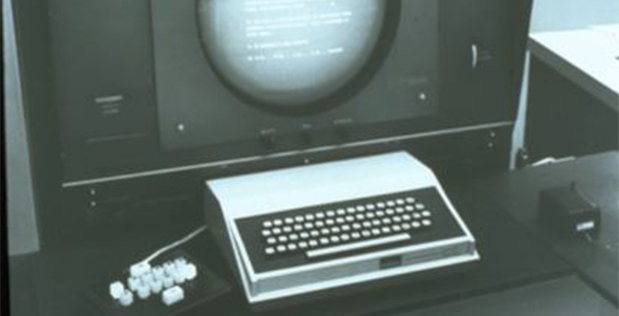
\includegraphics[width=0.8\textwidth]{nls.jpg}
        \caption{Daglas Engelbart tokom "Majke svih demonstracija", 1968.}
        \label{fig:nls_demo}
    \end{figure}

    
    Iako NLS nije bio kolaborativni editor u savremenom smislu, predstavljao je revolucionaran koncept koji je omogućavao zajedničko pregledanje i uređivanje dokumenata. Ovaj sistem je pokazao kako bi računar mogao postati alat za grupni rad, posebno u organizacijama sa složenim informacionim potrebama. Engelbartova vizija o umreženoj saradnji postavila je temelj za dalji razvoj kolaborativnih editora, ali su tehnološka ograničenja tog vremena sprečila njegovu široku primenu.
    
    U toku 1970-ih i ranih 1980-ih, nekoliko naučnih radova i istraživanja pokušalo je da reši problem zajedničkog uređivanja dokumenata. Međutim, zbog ograničenih mrežnih kapaciteta i činjenice da internet još uvek nije bio široko dostupan, razvoj je bio fokusiran na lokalne mreže i eksperimentalne sisteme. Primer toga bio je konceptualni okvir poznat kao \textbf{"Shared Workspace"}, koji je omogućavao korisnicima da dele radno okruženje i informacije u realnom vremenu. Ovi rani sistemi su omogućavali deljenje sadržaja, ali nisu nudili dinamičko uređivanje, koje je karakteristično za modernu kolaboraciju.

    \paragraph{}
    Tokom kasnih 1980-ih, tehnologija je značajno napredovala, a računarstvo je postajalo sve moćnije i pristupačnije. Ova era je videla pojavu prvih pravih kolaborativnih editora. Jedan od prvih sistema koji je omogućio više korisnika da uređuju dokumente u realnom vremenu bio je \textbf{GROVE (Group Outline Viewing Editor)}, razvijen 1989. godine. GROVE je omogućavao simultano uređivanje strukturisanih dokumenata i predstavljao je jedan od pionirskih sistema za kolaborativno uređivanje. Iako je bio ograničen na lokalne mreže, zbog nedostatka interneta i infrastrukture za širu mrežnu primenu, GROVE je pokazao kako bi kolaboracija mogla funkcionisati u okruženju sa više korisnika.

    GROVE omogućava prikazivanje više pogleda na konturu, gde se svaki prikaz prikazuje u grupnom prozoru koji može biti repliciran na više mašina. Ovi prikazi mogu biti privatni, deljeni ili javni, u zavisnosti od potreba korisnika. Značajna karakteristika GROVE sistema je njegov grupni prozor, koji prikazuje prisustvo i aktivnost svih učesnika koji rade na dokumentu. U ovom zajedničkom prostoru korisnici mogu izvršavati standardne operacije uređivanja, kao što su umetanje, brisanje, sečenje i lepljenje teksta. Sistem takođe nudi napredne funkcionalnosti, poput proširivanja i skupljanja delova konture, kao i promene dozvola za čitanje i pisanje specifičnih stavki.

    \begin{figure}[h]
        \centering
        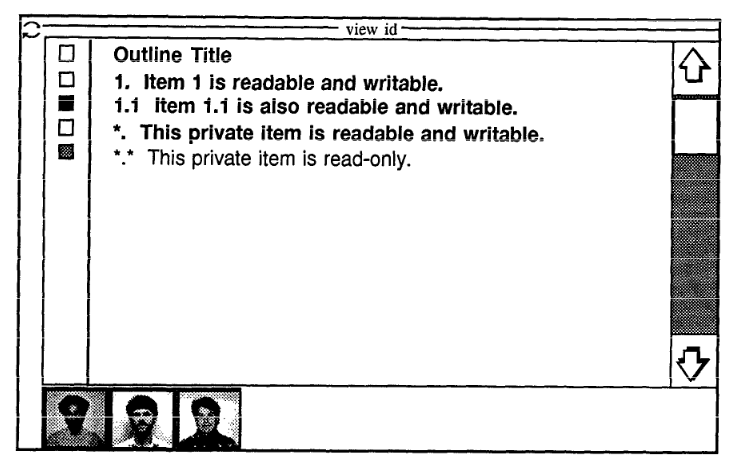
\includegraphics[width=0.8\textwidth]{grove.png}
        \caption{Grove grupni prozor, 1989.}
        \label{fig:nls_demo}
    \end{figure}

    Jedna od ključnih karakteristika GROVE sistema je kolaboracija u realnom vremenu—svaka promena koju napravi jedan učesnik odmah je vidljiva ostalima, osiguravajući da svi učesnici budu u toku sa najnovijim izmenama. Ovaj mehanizam povratne informacije u realnom vremenu bio je od suštinskog značaja za kreiranje visoko interaktivnog i responzivnog okruženja.
    
    Za razliku od sistema u realnom vremenu kao što je GROVE, drugi sistemi tog vremena, poput CES-a, Quilta ili Shared Books-a, omogućavali su kolaborativno uređivanje dokumenata, ali su radili u asinhronom režimu. Ovi sistemi su dozvoljavali korisnicima da rade na različitim delovima dokumenta, često tokom dužih perioda, što je omogućavalo manje fokusirane sesije. Distinkcija između kolaborativnih sistema u realnom i asinhronom vremenu postala je važan fokus u proučavanju kolaborativnih sistema.
    
    GROVE-ova mogućnost uređivanja u realnom vremenu, uz podršku za upravljanje različitim prikazima i korisničkim dozvolama, učinila ga je značajnim korakom u razvoju sistema za grupni rad.
    
    Pored GROVE-a, nekoliko drugih projekata je nastalo u ovom periodu, ali su svi imali slične izazove – mrežna infrastruktura nije bila dovoljno razvijena za globalnu kolaboraciju, a računarstvo nije bilo dovoljno moćno da podrži složene algoritme potrebne za rešavanje problema sinkronizacije i konzistentnosti podataka među korisnicima.
    
    Dakle, tokom 1970-ih i 1980-ih godina, iako su načinjeni značajni koraci u pravcu kolaborativnih sistema, ovi rani pokušaji su uglavnom ostali ograničeni na istraživačke laboratorije i specifične upotrebe unutar lokalnih mreža. Tek kasnije, sa razvojem interneta i većom dostupnošću mrežnih resursa, kolaborativni editori su počeli da ostvaruju svoj puni potencijal.

    \subsubsection{Razvoj real-time kolaboracije (2000-te)}

    Početak 2000-ih godina doneo je velike promene u načinu na koji ljudi rade zajedno, zahvaljujući razvoju interneta i novih tehnologija za kolaborativno uređivanje. Prethodne decenije, kolaborativni editori su postojali, ali su bili uglavnom ograničeni na lokalne mreže i zahtevali su specifične softverske sisteme. Sa ekspanzijom interneta, pojavile su se mogućnosti za udaljenu, real-time saradnju, što je omogućilo korisnicima da rade na istom dokumentu bez obzira na to gde se nalaze.

    Jedan od prvih značajnih sistema koji je omogućio ovakvu vrstu saradnje bio je SubEthaEdit, predstavljen 2003. godine. SubEthaEdit je bio jednostavan tekstualni editor za macOS, koji je omogućavao više korisnika da istovremeno uređuju isti dokument preko mreže. Ovaj alat je postao popularan među korisnicima macOS-a zbog svoje jednostavnosti i efikasnosti u real-time kolaboraciji. SubEthaEdit je označio početak šire dostupnosti kolaborativnih alata za svakodnevne korisnike.
    
    Međutim, pravi proboj u ovoj oblasti dogodio se 2006. godine sa lansiranjem Google Docs platforme. Google Docs je bio revolucionaran u tome što je omogućio korisnicima da kreiraju i uređuju dokumente u oblaku, a svi učesnici su mogli da prate promene u realnom vremenu. Ovo je značilo da su više ljudi mogli istovremeno da rade na istom dokumentu, dok su izmene bile odmah vidljive svima. Takva funkcionalnost je do tada bila retka i skupa, a Google je ovu tehnologiju učinio dostupnom besplatno, čime je pokrenuo masovnu upotrebu real-time kolaboracije.
    
    Google Docs je iskoristio prednosti cloud infrastrukture, što je omogućilo da dokumenti budu sačuvani na udaljenim serverima, dostupni s bilo kog uređaja sa internet konekcijom. Ovaj pristup je eliminisao potrebu za lokalnim skladištenjem i omogućio je lako deljenje dokumenata među korisnicima. Alat je omogućio istovremeno uređivanje, komentarisanje i komunikaciju unutar dokumenata, što je dramatično ubrzalo procese zajedničkog rada, posebno u obrazovnim, poslovnim i kreativnim sektorima.
    
    Pored Google Docs-a, pojavili su se i drugi alati poput Etherpad-a (2008) koji je bio otvorenog koda i pružao slične funkcionalnosti za kolaborativno uređivanje u realnom vremenu. Etherpad je bio popularan među zajednicama otvorenog koda jer je omogućavao korisnicima da pokreću svoje sopstvene instance servera za kolaborativno uređivanje, pružajući fleksibilnost u korišćenju.
    
    Tokom ovog perioda, koncept kolaborativnog rada postao je centralni deo produktivnosti na internetu. Dok su Google Docs i slični alati omogućavali ljudima da zajedno pišu dokumente, paralelno su se razvijali i drugi oblici kolaborativnih platformi, poput Wikija i Trello-a, koji su se fokusirali na organizaciju i saradnju na projektima.
    
    Real-time kolaboracija je tokom 2000-ih evoluirala od jednostavnih tekstualnih editora do kompleksnih platformi koje omogućavaju ne samo zajedničko pisanje, već i komunikaciju, deljenje resursa, planiranje i upravljanje projektima. Ovaj period označava prekretnicu u razvoju kolaborativnih tehnologija, postavljajući temelje za današnje sofisticirane alate koji se koriste širom sveta u raznim industrijama.

   \subsubsection{Moderni kolaborativni editori (2010-)}

   
    Moderni kolaborativni editori od 2010. godine pa nadalje nude napredne funkcionalnosti, prvenstveno u real-time kolaboraciji, gde više korisnika može simultano uređivati isti dokument ili projekat bez prekida u radu. Ovi alati koriste cloud infrastrukturu i napredne algoritme za sinhronizaciju, što omogućava momentalnu vidljivost unetih izmena za sve učesnike.
    
    \textbf{Karakteristike modernih kolaborativnih editora:}
    \begin{itemize}
        \item \textbf{Real-time kolaboracija} – Korisnici mogu simultano raditi na istim dokumentima, kodu ili projektu, a promene su odmah vidljive svim učesnicima.
        \item \textbf{Kolaborativne funkcije} – Uključuju mogućnost komentarisanja, dodeljivanja zadataka, praćenja revizija, kao i obaveštenja o aktivnostima drugih korisnika.
        \item \textbf{Rad na različitim uređajima} – Ovi alati su obično dostupni na više platformi (desktop, mobilni, tablet), što omogućava kolaboraciju s bilo koje lokacije.
        \item \textbf{Integracije} – Moderni alati često dolaze s integracijama za komunikaciju (npr. Slack), menadžment projekata (npr. Trello), i druge aplikacije koje olakšavaju rad.
        \item \textbf{Napredna kontrola verzija} – Sistemi za praćenje promena omogućavaju vraćanje na prethodne verzije i pregled ko je i kada izvršio određene izmene.
    \end{itemize}
    
    \textbf{Primeri modernih real-time kolaborativnih editora:}
    
    \paragraph{Figma}  
    je kolaborativni alat za dizajn koji omogućava real-time uređivanje i deljenje dizajn projekata. Figma omogućava dizajnerima, programerima i menadžerima da rade zajedno na interaktivnim prototipovima, s momentalnim uvidom u promene.

    \begin{figure}[h]
        \centering
        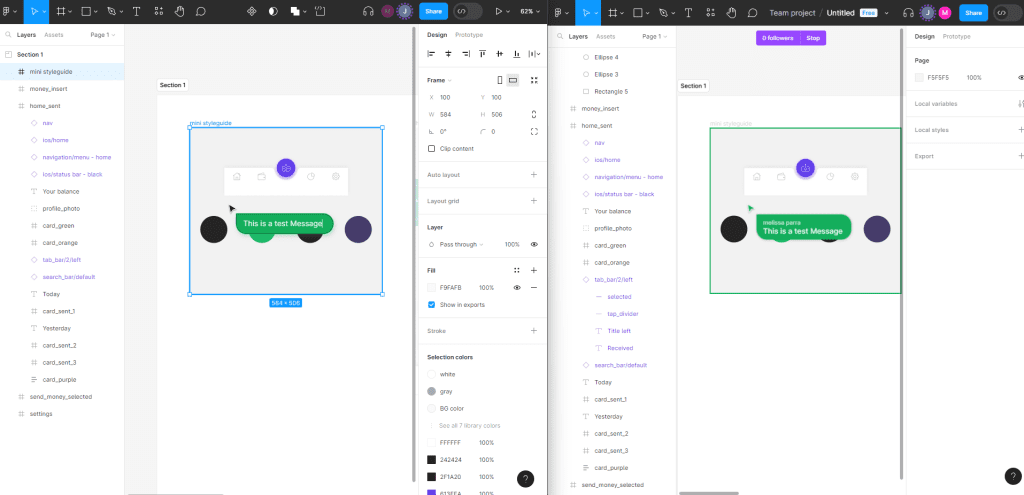
\includegraphics[width=0.8\textwidth]{figma.png}
        \caption{Alat za kolaboraciju Figma}
        \label{fig:nls_demo}
    \end{figure}
    
    \paragraph{Notion}  
    je platforma za beleške i upravljanje projektima koja se koristi za kolaboraciju u realnom vremenu. Korisnici mogu da kreiraju i uređuju stranice, dodaju zadatke, tabele i baze podataka, dok istovremeno više korisnika može da pristupa i uređuje iste sadržaje.
    
    \paragraph{Overleaf}  
    je web-bazirana LaTeX platforma koja omogućava kolaborativno uređivanje tehničkih dokumenata, akademskih radova, i istraživačkih radova. Idealna je za naučne i tehničke projekte, gde više korisnika simultano piše i uređuje dokumente u LaTeX-u, s momentalnim prikazom rezultata. Pomoću Overleaf-a je napisan i ovaj diplomski rad.
    
    Ovi alati predstavljaju ključne primere kako moderni editori omogućavaju bržu i efikasniju kolaboraciju, smanjujući potrebu za ručnom sinhronizacijom i olakšavajući zajednički rad na projektima.


    \startnewsection
    

    
    
\end{document}

